\documentclass[12pt]{article}
\usepackage[margin=1in]{geometry}
\usepackage{graphicx}

\begin{document}

\title {Observing the Sun, Moon, Orion and Crab Nebula using a
  two-element interferometer}
\author {Marta Pastore}
\date {March 7, 2014}
\maketitle

\begin {abstract}


\end {abstract}
Using an two-element inteferometer we observed the Sun, Moon, Orion and
the Crab Nebula. From the data obtained for the Crab Nebula we applied
least squares filling to determine the best guess for our baseline which
resulted to be around 8 meters. Similarly, least-fitting the data from
the Sun, we obtained the phase differance between the two antennas and
this resulted to be around 0.2 radians. 

\section {Introduction}

In this lab we focus on understanding basic interferometry.  We used two
antennas to obtain observational data from the Sun, moon and
Orion. These are all considered continuum sources so our telescopes are
able to detect them. We wrote a computer script that would allow us to
position the antennas in the right direction for each
source. Observations were taken from Horizon to horizon for the moon and
the sun. Orion was observed for a couple of hours. The method of least
square fitting was used to obtain information like the size of our
baseline, the radius of the Sun and moon and the declination of our
point source, Orion. 

\section {Methods}

For the gathering of the data we used two antennas located on the roof of
a building. This technique is called interferometry and it is very
commonly used in Radio Astronomy. We wrote a computed program that
controlled where the atennas point in order to obtain our
data. Determining the location of our sources of interest was very
import in the accuracy of our results. We then analyzed the data using a
method of least-square fitting. This allowed us to determine the radius
of Sun and Moon and also the declination of Orion. 

\subsection {Interferometer}
An interferometer consists of two antennas separated by some distance
called a baseline. The two antennas collect a signal which is then
processed through a complicated circuit to give a graph on the
computer. The graph that results from the interferometer is called a
fringe pattern and it represents the complex response of the baseline
along the sky. The fringe pattern looks very close to a sine
wave. Therefore, in our observation we expect to see a fringe pattern
that looks a bit like a sine wave for each source. 

The interferometer we used operates at about 11GHz. It has a short
baseline and the fringe spacing is large than the size of all sources,
except when we observe the Sun and Moon, so they can be considered as
point sources. 

Because the Sun is the brightest object in the sky, it is easy to obtain
a clear fringe pattern. this is why we determine the value of our
baseline from the Sun observations. With the baseline value, the fringe
properties represent the declination of the point-source which in our
case is Orion.  Our baseline is  10m and this means we have a fringe
spacing of 10' and with a horizon-to-horizon observation we can measure
the declination more accurately. This is precisely why we are taking
horizon-to-horizon measurements for the Sun and Moon. From this
observation of the Sun and Moon we can measure their diameters to a
fraction of a percent. 

The way our interferometer works is it takes the two signals from each
telescope and multiplies them together via a mixer. The data we end up
recording is the time average of the product of the signals over a time
interval of a few seconds. The multiplication of the two signals is done
through a cross product because this allows the average value to be zero
unless there is a source. This ensure us that any detected signal is
coming from the source only. For a particular source, the fringe
amplitude has no zero offset and it is directly proportional to the
source flux. 


\subsection {Rotational Matrices}

In order to get our observations we need to know the azimuth and
altitude of the source so that the telescopes can know where to
point. The azimuth and altitude of the Sun and Moon can easily be
obtained at any given time using the PyEphem module. However, The
azimuth and altitude can also be calculated using a rotational matrix,
R, and the values for the sources right ascension and declination. The
way the rotational matrix works is by you dotting the matrix containing
the values of the right ascension and declination for a source with the
rotational matrix R to give a resulting matrix containing the values of
the azimuth and altitude for that source. In our case, the Sun and Moon
have a changing right ascension and declination therefore we have to
account for the changes in position with time. For our point source
Orion there is a set value for the right ascension and declination. 

\subsection {Least-Squares Fitting}

Least-squares fitting is a method for approximating the solution for a
set of data. In our case we are using this method for the approximation
of Moon and Sun radius as well as the declination of our point
source. In order to do this, we start by reading a data file and
transferring the numbers to a matrix using IDL commands. What follows
are a series of steps that will allow us to plot our data fitted to the
approximate solution which in our case is a sine wave. With this plot we
have the necessary information to determine the approximate radius of
the Sun and Moon.

\section {Results and Discussion}

We observed the Sun and Moon from horizon-to-horizon and Orion and the
crab nebula for approximately 4 hours. From this a plot of voltage vs
time was obtained for each source.
\subsection {Orion and Crab Nebula Observation Results}
The signal for Orion and Crab Nebula are show in Figure 1 and 2. For
Orion we have a bit of strange data in the beginning but it ends up
becoming steady after some time. The voltage seems to stay between
-0.0005 and -0.0010 volts. The negative voltage/power values come from
the fringe pattern of the source. For the Crab Nebula the data around
the middle of Figure 2 is what we expect. Then parts where the voltage
fluctuates a lot must be due to some inteferance. From this plot of the
Crab Nebula, we applied least square fitting in order to get the best
guess for the baseline of our telescopes. We did this by guessing
different values for the baseline and calculating the error of each
value. A plot of this is show in Figure 3. In this figure we look for the
minimum y value and the corresponding x value is our best guess for the
baseline. We therefore conclude that the baseline is around 8 meters.

\begin {figure}[h!]
\centering
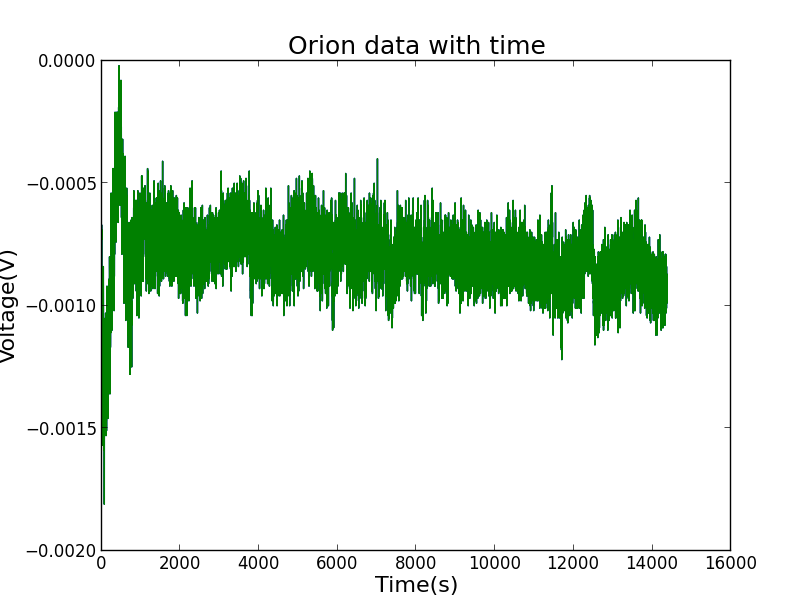
\includegraphics[scale = 0.5]
{orionwithtime.png}
\caption{\label{rvd} A plot of the signal of Orion with time using an interferometer.}
\end {figure}

\begin {figure}[h!]
\centering
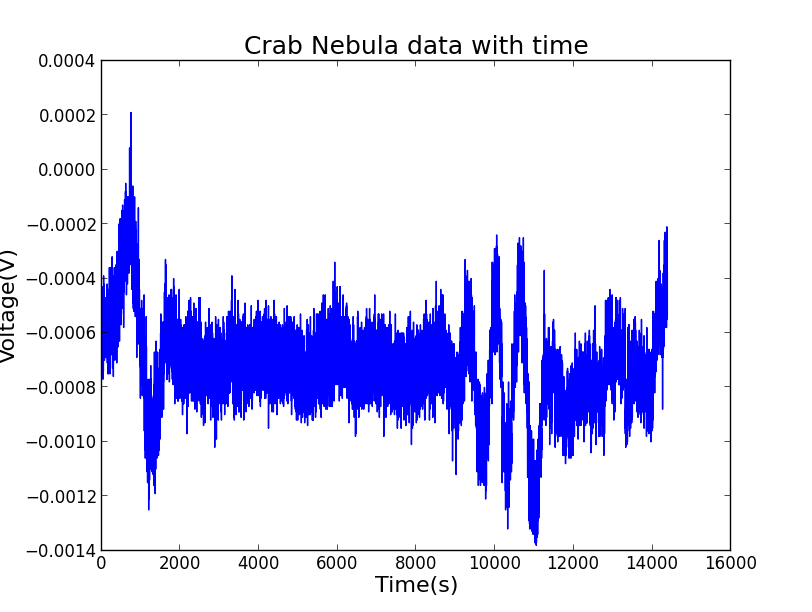
\includegraphics[scale = 0.5]
{crabwithtime.png}
\caption{\label{rvd} A plot of the Crab Nebula signal with time using an interferometer}
\end {figure}

\begin {figure}[h!]
\centering
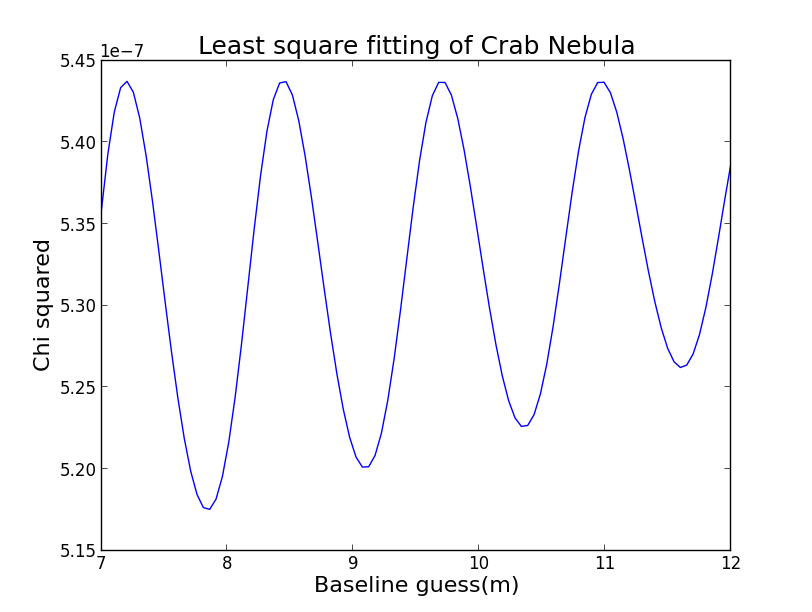
\includegraphics[scale = 0.5]
{chisquaredcrab.png}
\caption{\label{rvd} The error associated with various
  guesses for the baseline of our interferometer.}
\end {figure}

\subsection {Sun Observation Results}

The Sun signal with respect to time is shown in Figure 4. If we zoom in
on this graph we can see the sine wave that represents our fringe
pattern. This is shown in Figure 5. The negative values of voltage or
power come from the fringe pattern. Unlike the point sources, we get a
pretty nice sine wave for the fringe patter because the Sun is so big
and bright in the sky, which is why the Sun was a great tested for our
script to control the telescopes. We went on to applying least square
fitting to the Sun data in order to find the phase differance of our
antennas. This phase difference, phi, comes from the fact that the
signal from one antenna differs for the other. This difference is
proportional to the baseline. The plot for the guesses for phi and their
corresponding error with our data is shown in Figure 6. We look for the
minimum value of y and the corresponding x value will give us the most
accurate phase differance. We can conclude that the best guess for the
phase differance is approximately 0.2 radians.

  
\begin {figure}[h!]
\centering
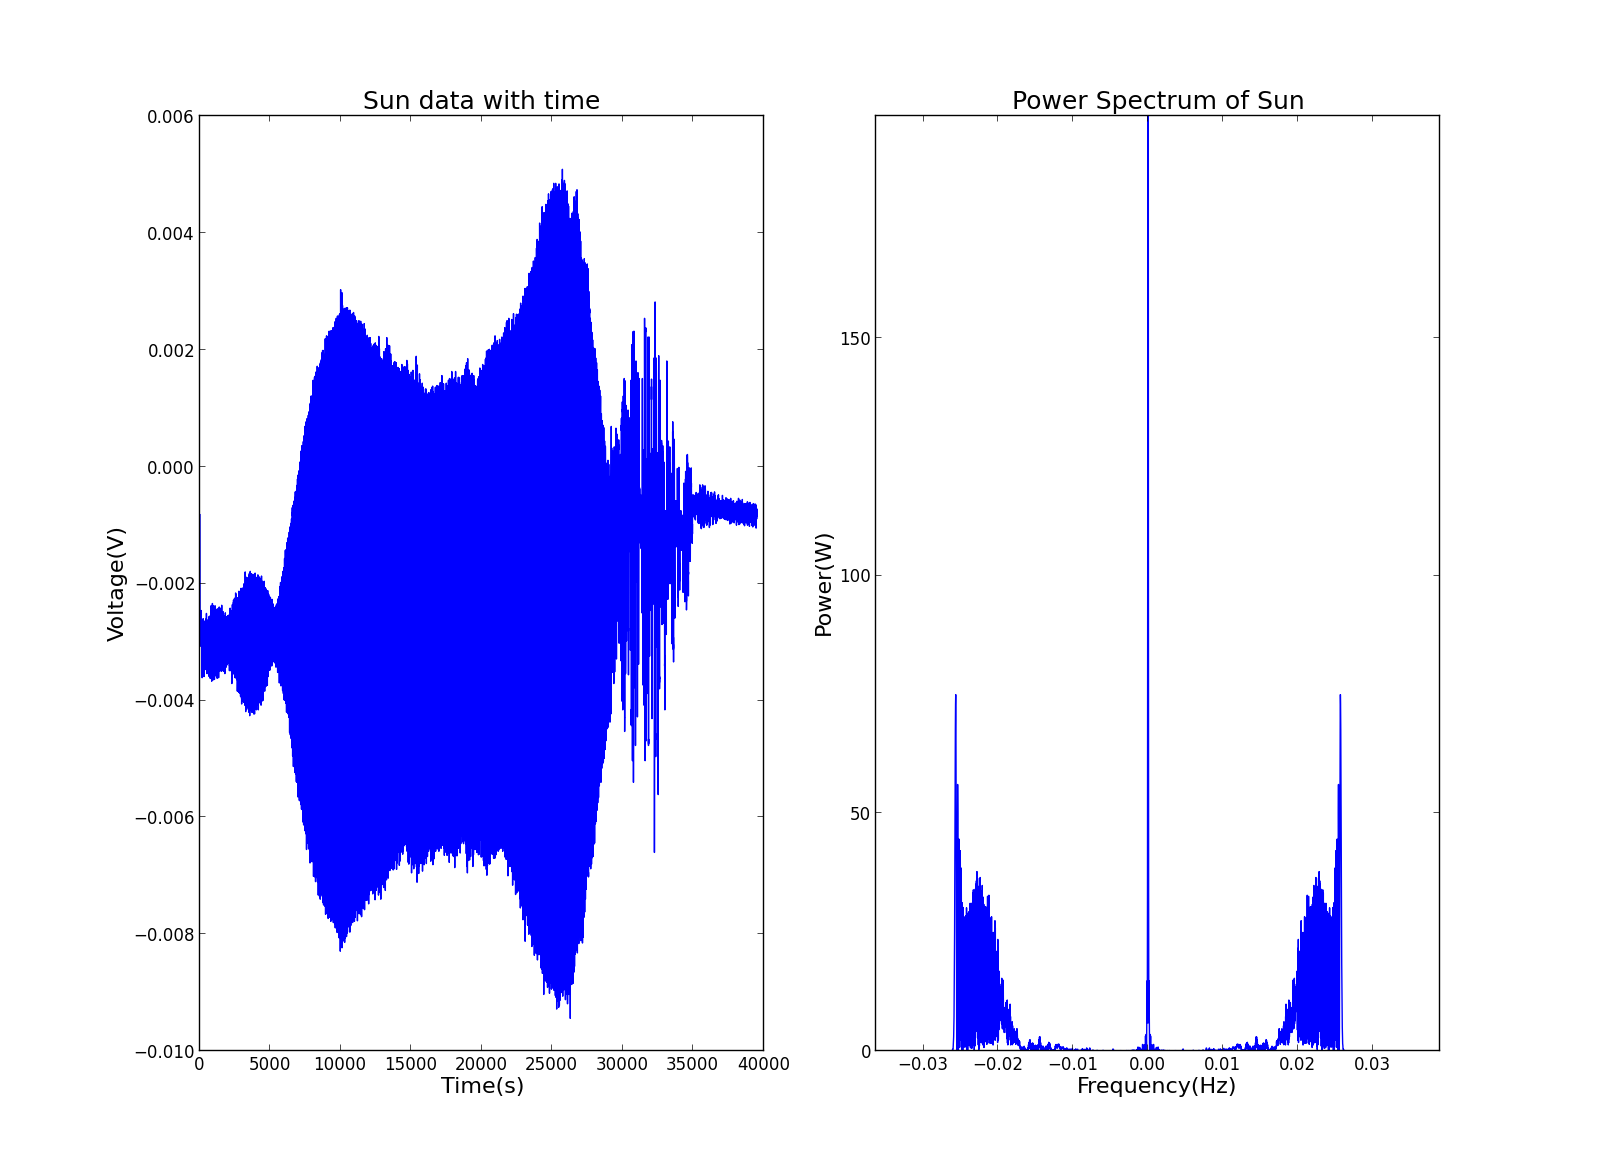
\includegraphics[scale = 0.5]
{sungraph1.png}
\caption{\label{rvd} A plot of the Sun signal from horizon-to-horizon
  using an interferometer}
\end {figure}

\begin {figure}[h!]
\centering
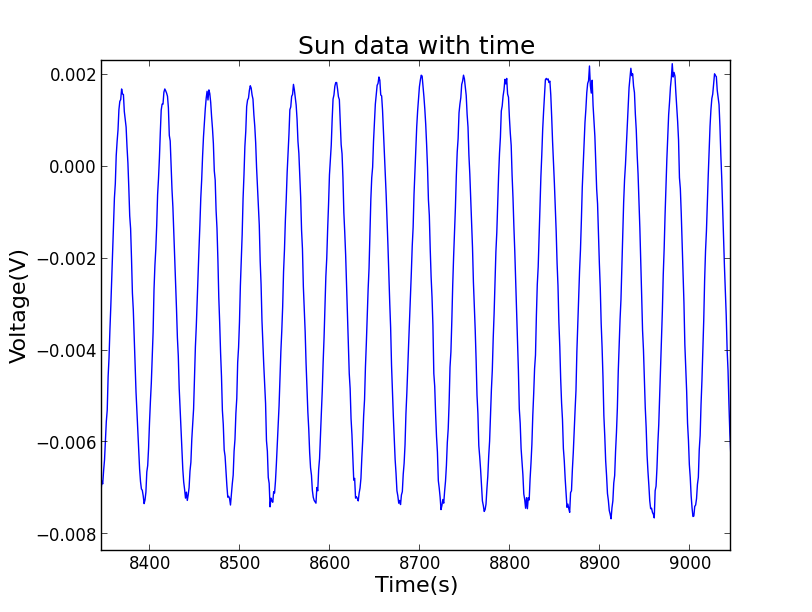
\includegraphics[scale = 0.5]
{zoomsun.png}
\caption{\label{rvd} A zoomed in vesion for the plot of the Sun signal
  form horizon-to-horizon using an interferometer}
\end {figure}

\begin {figure}[h!]
\centering
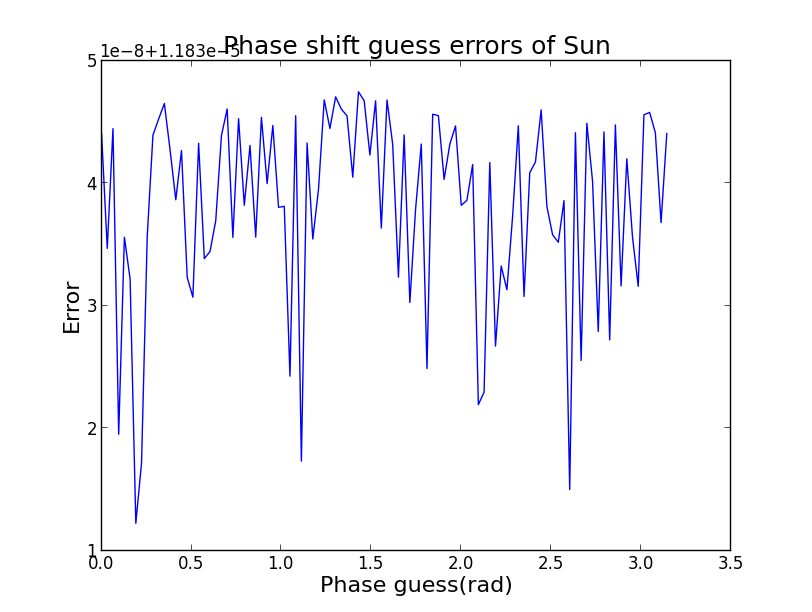
\includegraphics[scale = 0.5]
{errorsun.png}
\caption{\label{rvd} The errors associated with various guesses for the
  phase difference, phi, for the Sun data.}
\end {figure}

\subsection {Moon Observation Results}
The signal for the horizon-horizon observation for the Moon are shown in
Figure 7. We would expect to the something a little better than what we
got because the Moon is so big. There is a lot of noise which can
result from the actual script used for the observation and the phase of
the moon. We still performed a least
square fitting to this data and this is shown in Figure 8. 

\begin {figure}[h!]
\centering
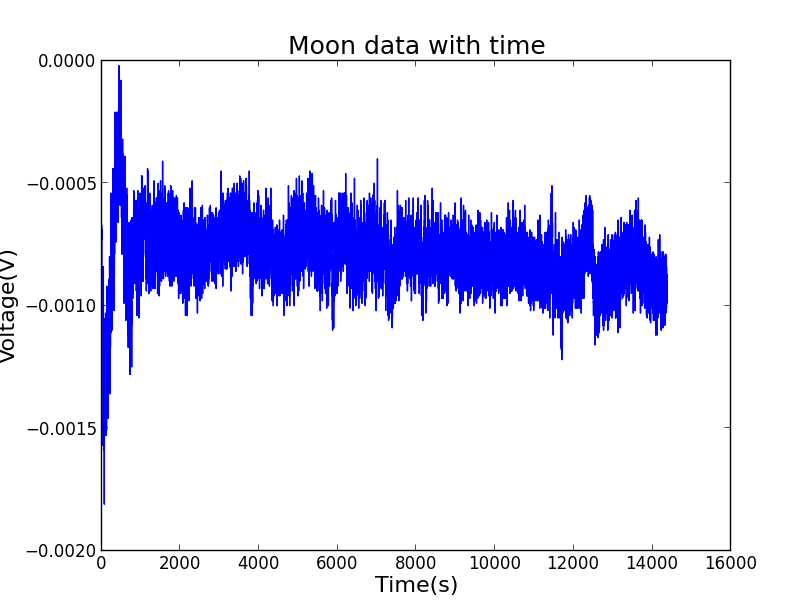
\includegraphics[scale = 0.5]
{moondatatime.png}
\caption{\label{rvd} A plot of the Moon signal from horizon-to-horizon
  using an interferometer}
\end {figure}

\begin {figure}[h!]
\centering
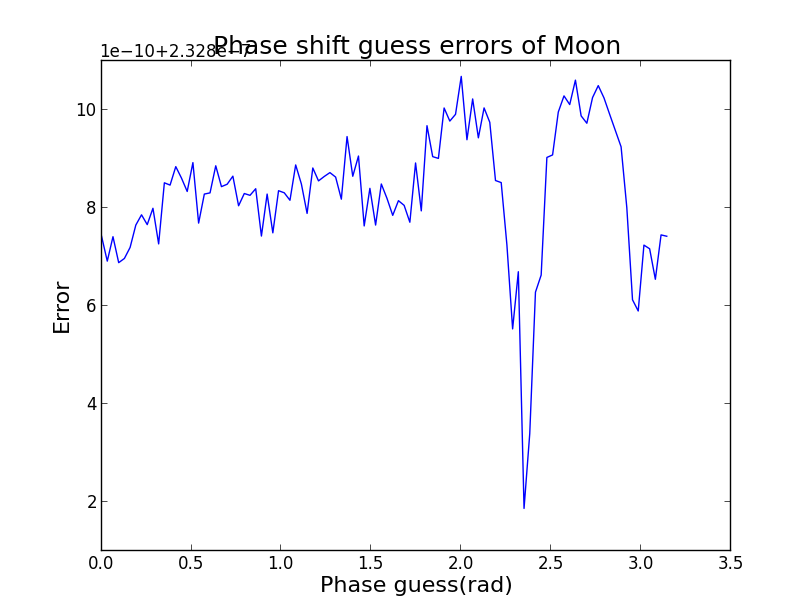
\includegraphics[scale = 0.5]
{errormoon.png}
\caption{\label{rvd} The errors associated with various guesses for the
  phase difference, phi, for the Moon data.}
\end {figure}




\section {Conclusion}
In this lab we were able to use least square fitting on the data from
the Crab Nebula to find the best guess for the baseline of our
antennas. In the future we would like to explore other information about
our data using least-square fitting like the radius of the Sun and
Moon. 

\section {Acknowledgements}
I would like to thank my group members Maissa Salama, Vikram Lyer, and
Dave Galbraith for their contribution in obtaining the data for this lab. I
would also like to thank Baylee Bordwell and Karto Keating for their
contribution in the analysis of the data. 

\end {document}
